\documentclass{standalone}
\usepackage{tikz}
\usetikzlibrary{patterns, positioning}


\begin{document}
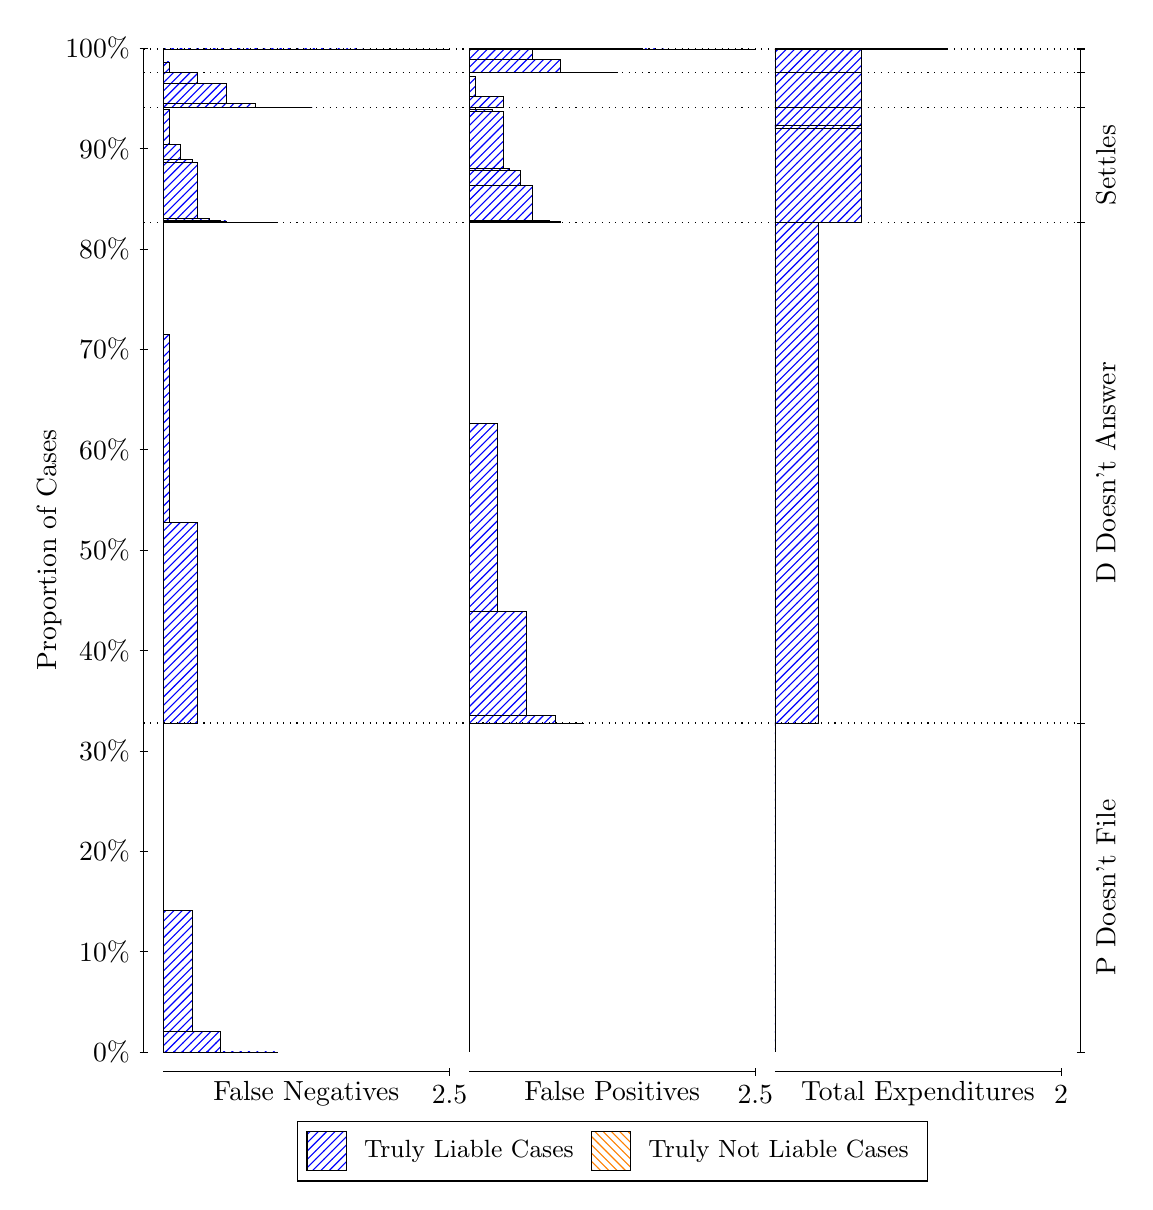
\begin{tikzpicture}
\draw[black, very thin] (1.5,1.75) -- (1.5,14.5);
\node[rotate=90, text=black, anchor=center] at (0.3, 8.125) {Proportion of Cases};
\draw[black, very thin] (1.45,1.75) -- (1.55,1.75);
\node[text=black, anchor=east] at (1.45, 1.75) {0\%};
\draw[black, very thin] (1.45,3.025) -- (1.55,3.025);
\node[text=black, anchor=east] at (1.45, 3.025) {10\%};
\draw[black, very thin] (1.45,4.3) -- (1.55,4.3);
\node[text=black, anchor=east] at (1.45, 4.3) {20\%};
\draw[black, very thin] (1.45,5.575) -- (1.55,5.575);
\node[text=black, anchor=east] at (1.45, 5.575) {30\%};
\draw[black, very thin] (1.45,6.85) -- (1.55,6.85);
\node[text=black, anchor=east] at (1.45, 6.85) {40\%};
\draw[black, very thin] (1.45,8.125) -- (1.55,8.125);
\node[text=black, anchor=east] at (1.45, 8.125) {50\%};
\draw[black, very thin] (1.45,9.4) -- (1.55,9.4);
\node[text=black, anchor=east] at (1.45, 9.4) {60\%};
\draw[black, very thin] (1.45,10.675) -- (1.55,10.675);
\node[text=black, anchor=east] at (1.45, 10.675) {70\%};
\draw[black, very thin] (1.45,11.95) -- (1.55,11.95);
\node[text=black, anchor=east] at (1.45, 11.95) {80\%};
\draw[black, very thin] (1.45,13.225) -- (1.55,13.225);
\node[text=black, anchor=east] at (1.45, 13.225) {90\%};
\draw[black, very thin] (1.45,14.5) -- (1.55,14.5);
\node[text=black, anchor=east] at (1.45, 14.5) {100\%};

\draw[black, very thin] (13.4,1.75) -- (13.4,14.5);
\draw[black, very thin] (13.35,1.75) -- (13.45,1.75);
\node[anchor=west] at (13.35, 1.75) {};
\draw[black, very thin] (13.35,5.9277) -- (13.45,5.9277);
\node[anchor=west] at (13.35, 5.9277) {};
\draw[black, very thin] (13.35,12.281) -- (13.45,12.281);
\node[anchor=west] at (13.35, 12.281) {};
\draw[black, very thin] (13.35,13.748) -- (13.45,13.748);
\node[anchor=west] at (13.35, 13.748) {};
\draw[black, very thin] (13.35,14.19) -- (13.45,14.19);
\node[anchor=west] at (13.35, 14.19) {};
\draw[black, very thin] (13.35,14.487) -- (13.45,14.487);
\node[anchor=west] at (13.35, 14.487) {};
\draw[black, very thin] (13.35,14.5) -- (13.45,14.5);
\node[anchor=west] at (13.35, 14.5) {};

\draw[black, very thin, pattern color=blue, pattern=north east lines] (1.75,1.75) rectangle (3.2033,1.75);
\draw[black, very thin, pattern color=blue, pattern=north east lines] (1.75,1.75) rectangle (2.84,1.7522);
\draw[black, very thin, pattern color=blue, pattern=north east lines] (1.75,1.7522) rectangle (2.4767,2.0161);
\draw[black, very thin, pattern color=blue, pattern=north east lines] (1.75,2.0161) rectangle (2.1133,3.5492);
\draw[black, very thin, pattern color=orange, pattern=north west lines] (1.75,3.5492) rectangle (1.75,3.5492);
\draw[black, very thin, pattern color=blue, pattern=north east lines] (1.75,3.5492) rectangle (1.75,5.9277);
\draw[black, very thin, pattern color=blue, pattern=north east lines] (1.75,5.9277) rectangle (2.186,8.4761);
\draw[black, very thin, pattern color=blue, pattern=north east lines] (1.75,8.4761) rectangle (1.8227,10.864);
\draw[black, very thin, pattern color=orange, pattern=north west lines] (1.75,10.864) rectangle (1.75,10.864);
\draw[black, very thin, pattern color=blue, pattern=north east lines] (1.75,10.864) rectangle (1.75,12.281);
\draw[black, very thin, pattern color=blue, pattern=north east lines] (1.75,12.281) rectangle (3.2033,12.281);
\draw[black, very thin, pattern color=blue, pattern=north east lines] (1.75,12.281) rectangle (3.058,12.281);
\draw[black, very thin, pattern color=blue, pattern=north east lines] (1.75,12.281) rectangle (2.9127,12.281);
\draw[black, very thin, pattern color=blue, pattern=north east lines] (1.75,12.281) rectangle (2.84,12.281);
\draw[black, very thin, pattern color=blue, pattern=north east lines] (1.75,12.281) rectangle (2.6947,12.281);
\draw[black, very thin, pattern color=blue, pattern=north east lines] (1.75,12.281) rectangle (2.5493,12.306);
\draw[black, very thin, pattern color=blue, pattern=north east lines] (1.75,12.306) rectangle (2.4767,12.308);
\draw[black, very thin, pattern color=blue, pattern=north east lines] (1.75,12.308) rectangle (2.3313,12.335);
\draw[black, very thin, pattern color=blue, pattern=north east lines] (1.75,12.335) rectangle (2.186,13.051);
\draw[black, very thin, pattern color=blue, pattern=north east lines] (1.75,13.051) rectangle (2.1133,13.087);
\draw[black, very thin, pattern color=blue, pattern=north east lines] (1.75,13.087) rectangle (1.968,13.274);
\draw[black, very thin, pattern color=blue, pattern=north east lines] (1.75,13.274) rectangle (1.8227,13.719);
\draw[black, very thin, pattern color=orange, pattern=north west lines] (1.75,13.719) rectangle (1.75,13.719);
\draw[black, very thin, pattern color=blue, pattern=north east lines] (1.75,13.719) rectangle (1.75,13.748);
\draw[black, very thin, pattern color=blue, pattern=north east lines] (1.75,13.748) rectangle (3.6393,13.748);
\draw[black, very thin, pattern color=blue, pattern=north east lines] (1.75,13.748) rectangle (3.276,13.748);
\draw[black, very thin, pattern color=blue, pattern=north east lines] (1.75,13.748) rectangle (2.9127,13.801);
\draw[black, very thin, pattern color=blue, pattern=north east lines] (1.75,13.801) rectangle (2.5493,14.047);
\draw[black, very thin, pattern color=blue, pattern=north east lines] (1.75,14.047) rectangle (2.186,14.19);
\draw[black, very thin, pattern color=orange, pattern=north west lines] (1.75,14.19) rectangle (1.75,14.19);
\draw[black, very thin, pattern color=blue, pattern=north east lines] (1.75,14.19) rectangle (2.186,14.191);
\draw[black, very thin, pattern color=blue, pattern=north east lines] (1.75,14.191) rectangle (1.8227,14.325);
\draw[black, very thin, pattern color=orange, pattern=north west lines] (1.75,14.325) rectangle (1.75,14.325);
\draw[black, very thin, pattern color=blue, pattern=north east lines] (1.75,14.325) rectangle (1.75,14.487);
\draw[black, very thin, pattern color=blue, pattern=north east lines] (1.75,14.487) rectangle (5.3833,14.487);
\draw[black, very thin, pattern color=blue, pattern=north east lines] (1.75,14.487) rectangle (5.02,14.487);
\draw[black, very thin, pattern color=blue, pattern=north east lines] (1.75,14.487) rectangle (4.6567,14.487);
\draw[black, very thin, pattern color=blue, pattern=north east lines] (1.75,14.487) rectangle (4.2933,14.49);
\draw[black, very thin, pattern color=blue, pattern=north east lines] (1.75,14.49) rectangle (3.93,14.49);
\draw[black, very thin, pattern color=blue, pattern=north east lines] (1.75,14.49) rectangle (3.5667,14.49);
\draw[black, very thin, pattern color=blue, pattern=north east lines] (1.75,14.49) rectangle (2.404,14.49);
\draw[black, very thin, pattern color=blue, pattern=north east lines] (1.75,14.49) rectangle (2.0407,14.49);
\draw[black, very thin, pattern color=orange, pattern=north west lines] (1.75,14.49) rectangle (1.75,14.49);
\draw[black, very thin, pattern color=blue, pattern=north east lines] (1.75,14.49) rectangle (1.75,14.5);
\draw[black, very thin, pattern color=orange, pattern=north west lines] (5.6333,1.75) rectangle (5.6333,1.75);
\draw[black, very thin, pattern color=blue, pattern=north east lines] (5.6333,1.75) rectangle (5.6333,5.9277);
\draw[black, very thin, pattern color=orange, pattern=north west lines] (5.6333,5.9277) rectangle (7.0867,5.9277);
\draw[black, very thin, pattern color=blue, pattern=north east lines] (5.6333,5.9277) rectangle (7.0867,5.9279);
\draw[black, very thin, pattern color=blue, pattern=north east lines] (5.6333,5.9279) rectangle (6.7233,6.0272);
\draw[black, very thin, pattern color=blue, pattern=north east lines] (5.6333,6.0272) rectangle (6.36,7.344);
\draw[black, very thin, pattern color=blue, pattern=north east lines] (5.6333,7.344) rectangle (5.9967,9.7323);
\draw[black, very thin, pattern color=blue, pattern=north east lines] (5.6333,9.7323) rectangle (5.6333,12.281);
\draw[black, very thin, pattern color=orange, pattern=north west lines] (5.6333,12.281) rectangle (6.796,12.281);
\draw[black, very thin, pattern color=blue, pattern=north east lines] (5.6333,12.281) rectangle (6.796,12.294);
\draw[black, very thin, pattern color=orange, pattern=north west lines] (5.6333,12.294) rectangle (6.6507,12.294);
\draw[black, very thin, pattern color=blue, pattern=north east lines] (5.6333,12.294) rectangle (6.6507,12.307);
\draw[black, very thin, pattern color=orange, pattern=north west lines] (5.6333,12.307) rectangle (6.5053,12.307);
\draw[black, very thin, pattern color=blue, pattern=north east lines] (5.6333,12.307) rectangle (6.5053,12.31);
\draw[black, very thin, pattern color=blue, pattern=north east lines] (5.6333,12.31) rectangle (6.4327,12.755);
\draw[black, very thin, pattern color=blue, pattern=north east lines] (5.6333,12.755) rectangle (6.2873,12.942);
\draw[black, very thin, pattern color=blue, pattern=north east lines] (5.6333,12.942) rectangle (6.142,12.978);
\draw[black, very thin, pattern color=blue, pattern=north east lines] (5.6333,12.978) rectangle (6.0693,13.694);
\draw[black, very thin, pattern color=blue, pattern=north east lines] (5.6333,13.694) rectangle (5.924,13.721);
\draw[black, very thin, pattern color=blue, pattern=north east lines] (5.6333,13.721) rectangle (5.7787,13.723);
\draw[black, very thin, pattern color=blue, pattern=north east lines] (5.6333,13.723) rectangle (5.706,13.748);
\draw[black, very thin, pattern color=blue, pattern=north east lines] (5.6333,13.748) rectangle (5.6333,13.748);
\draw[black, very thin, pattern color=orange, pattern=north west lines] (5.6333,13.748) rectangle (6.0693,13.748);
\draw[black, very thin, pattern color=blue, pattern=north east lines] (5.6333,13.748) rectangle (6.0693,13.89);
\draw[black, very thin, pattern color=blue, pattern=north east lines] (5.6333,13.89) rectangle (5.706,14.136);
\draw[black, very thin, pattern color=blue, pattern=north east lines] (5.6333,14.136) rectangle (5.6333,14.19);
\draw[black, very thin, pattern color=orange, pattern=north west lines] (5.6333,14.19) rectangle (7.5227,14.19);
\draw[black, very thin, pattern color=blue, pattern=north east lines] (5.6333,14.19) rectangle (7.5227,14.19);
\draw[black, very thin, pattern color=blue, pattern=north east lines] (5.6333,14.19) rectangle (7.1593,14.192);
\draw[black, very thin, pattern color=blue, pattern=north east lines] (5.6333,14.192) rectangle (6.796,14.351);
\draw[black, very thin, pattern color=blue, pattern=north east lines] (5.6333,14.351) rectangle (6.4327,14.485);
\draw[black, very thin, pattern color=blue, pattern=north east lines] (5.6333,14.485) rectangle (6.0693,14.487);
\draw[black, very thin, pattern color=orange, pattern=north west lines] (5.6333,14.487) rectangle (9.2667,14.487);
\draw[black, very thin, pattern color=blue, pattern=north east lines] (5.6333,14.487) rectangle (9.2667,14.487);
\draw[black, very thin, pattern color=orange, pattern=north west lines] (5.6333,14.487) rectangle (8.9033,14.487);
\draw[black, very thin, pattern color=blue, pattern=north east lines] (5.6333,14.487) rectangle (8.9033,14.487);
\draw[black, very thin, pattern color=orange, pattern=north west lines] (5.6333,14.487) rectangle (8.54,14.487);
\draw[black, very thin, pattern color=blue, pattern=north east lines] (5.6333,14.487) rectangle (8.54,14.487);
\draw[black, very thin, pattern color=orange, pattern=north west lines] (5.6333,14.487) rectangle (8.1767,14.487);
\draw[black, very thin, pattern color=blue, pattern=north east lines] (5.6333,14.487) rectangle (8.1767,14.49);
\draw[black, very thin, pattern color=blue, pattern=north east lines] (5.6333,14.49) rectangle (7.8133,14.496);
\draw[black, very thin, pattern color=blue, pattern=north east lines] (5.6333,14.496) rectangle (7.45,14.497);
\draw[black, very thin, pattern color=blue, pattern=north east lines] (5.6333,14.497) rectangle (7.0867,14.497);
\draw[black, very thin, pattern color=blue, pattern=north east lines] (5.6333,14.497) rectangle (6.7233,14.497);
\draw[black, very thin, pattern color=orange, pattern=north west lines] (5.6333,14.497) rectangle (5.6333,14.497);
\draw[black, very thin, pattern color=blue, pattern=north east lines] (5.6333,14.497) rectangle (5.6333,14.5);
\draw[black, very thin, pattern color=orange, pattern=north west lines] (9.5167,1.75) rectangle (9.5167,1.75);
\draw[black, very thin, pattern color=blue, pattern=north east lines] (9.5167,1.75) rectangle (9.5167,5.9277);
\draw[black, very thin, pattern color=orange, pattern=north west lines] (9.5167,5.9277) rectangle (10.062,5.9277);
\draw[black, very thin, pattern color=blue, pattern=north east lines] (9.5167,5.9277) rectangle (10.062,12.281);
\draw[black, very thin, pattern color=orange, pattern=north west lines] (9.5167,12.281) rectangle (10.607,12.281);
\draw[black, very thin, pattern color=blue, pattern=north east lines] (9.5167,12.281) rectangle (10.607,13.48);
\draw[black, very thin, pattern color=orange, pattern=north west lines] (9.5167,13.48) rectangle (10.607,13.48);
\draw[black, very thin, pattern color=blue, pattern=north east lines] (9.5167,13.48) rectangle (10.607,13.521);
\draw[black, very thin, pattern color=orange, pattern=north west lines] (9.5167,13.521) rectangle (10.607,13.521);
\draw[black, very thin, pattern color=blue, pattern=north east lines] (9.5167,13.521) rectangle (10.607,13.748);
\draw[black, very thin, pattern color=orange, pattern=north west lines] (9.5167,13.748) rectangle (10.607,13.748);
\draw[black, very thin, pattern color=blue, pattern=north east lines] (9.5167,13.748) rectangle (10.607,14.19);
\draw[black, very thin, pattern color=orange, pattern=north west lines] (9.5167,14.19) rectangle (10.607,14.19);
\draw[black, very thin, pattern color=blue, pattern=north east lines] (9.5167,14.19) rectangle (10.607,14.487);
\draw[black, very thin, pattern color=orange, pattern=north west lines] (9.5167,14.487) rectangle (11.697,14.487);
\draw[black, very thin, pattern color=blue, pattern=north east lines] (9.5167,14.487) rectangle (11.697,14.5);
\draw[black, dotted] (1.5,5.9277) -- (13.4,5.9277);
\draw[black, dotted] (1.5,12.281) -- (13.4,12.281);
\draw[black, dotted] (1.5,13.748) -- (13.4,13.748);
\draw[black, dotted] (1.5,14.19) -- (13.4,14.19);
\draw[black, dotted] (1.5,14.487) -- (13.4,14.487);
\draw[black, very thin] (1.75,1.5) -- (5.3833,1.5);
\node[text=black, anchor=north] at (3.5667, 1.5) {False Negatives};
\draw[black, very thin] (5.3833,1.45) -- (5.3833,1.55);
\node[text=black, anchor=north] at (5.3833, 1.45) {2.5};

\draw[black, very thin] (5.6333,1.5) -- (9.2667,1.5);
\node[text=black, anchor=north] at (7.45, 1.5) {False Positives};
\draw[black, very thin] (9.2667,1.45) -- (9.2667,1.55);
\node[text=black, anchor=north] at (9.2667, 1.45) {2.5};

\draw[black, very thin] (9.5167,1.5) -- (13.15,1.5);
\node[text=black, anchor=north] at (11.333, 1.5) {Total Expenditures};
\draw[black, very thin] (13.15,1.45) -- (13.15,1.55);
\node[text=black, anchor=north] at (13.15, 1.45) {2};

\node[text=black, centered, rotate=90] at (13.72, 3.8389) {P Doesn't File};
\node[text=black, centered, rotate=90] at (13.72, 9.1042) {D Doesn't Answer};
\node[text=black, centered, rotate=90] at (13.72, 13.014) {Settles};




\draw (7.449999999999999,1.5) node[draw=none] (baseCoordinate) {};
\begin{scope}[align=center]
        \matrix[scale=0.5, draw=black, below=0.5cm of baseCoordinate, nodes={draw}, column sep=0.1cm]{
            \node[rectangle, draw, minimum width=0.5cm, minimum height=0.5cm, pattern color=blue, pattern=north east lines] {}; &
            \node[draw=none, font=\small, text=black] (B) {Truly Liable Cases}; &
            \node[rectangle, draw, minimum width=0.5cm, minimum height=0.5cm, pattern color=orange, pattern=north west lines] {}; &
            \node[draw=none, font=\small, text=black] (B) {Truly Not Liable Cases}; \\
            };
\end{scope}

\end{tikzpicture}
\end{document}